\mychapter{Resultados Experimentais}
\label{Cap:Resultados}

Antes mesmo de testar a qualidade da comunicação dos módulos XBee em chão, foram realizados testes de comportamento do aeromodelo \emph{Phantom} quanto a possível interferência que a rede formada pelos XBees poderia causar na comunicação entre o mesmo e o controle remoto, afim de garantir a integridade de ambos os equipamentos envolvidos. Certificou-se, então, que o funcionamento da aeronave em nada era afetado com a presença da rede XBee.

\section{Teste em Solo}

Para a análise da qualidade da rede XBee em solo, foram realizados três testes de potência do sinal a três diferente distâncias, sendo elas 50, 100 e 236. Para cada teste foram enviados 40 pacotes de dados com metade da capacidade máxima de \emph{payload}, ou seja, 32 \emph{bytes}. Como mostra a Figura \ref{fig:SuccessChao}, a taxa de sucesso de envio de pacotes cai de aproximadamente 95 por cento para 5 por cento entre as distâncias de 100 e 236 metros, praticamente eliminando o \emph{link} de comunicação entre os dois nós da rede.

Para os testes realizados com 236 metros de afastamento entre os nós, nas quarenta tentativas de envio de pacote entre os nós da rede, trinta e oito delas acusaram \emph{TX Errors}, o que significa que o nó remetente não foi capaz de criar o \emph{link} de comunicação com o nó destinatário do pacote, resultando assim em apenas duas transmissões de dados bem sucedidas, resultando na taxa de sucesso de 5 por cento.

Quanto ao teste da taxa de transmissão de dados, foram realizados apenas dois testes sendo o primeiro com 50 metros de afastamento entre os nós e o segundo com 100 metros. Para a terceira distância, sendo essa 236 metros, foi impossível a realização do teste de taxa de transferência devido a má qualidade de comunicação. Os resultados desses dois testes podem ser vistos na Figura \ref{fig:ThroughputChao}.

O resultado de ambos os testes de força de sinal e taxa de transmissão não corresponderam ao esperado. Como os testes foram realizados no campo central da UFRN, considera-se área urbana, esperava-se que os módulos tivessem um desempenho próxima à indicada no manual do equipamento, que seria um alcance de aproximadamente 610 metros com uma taxa de transmissão de 10 kbps, ou 305 metros com uma taxa de transmissão de 200 kbps. Em contra partida, a comunicação entre os nós já foi comprometida à aproximadamente 235 metros e a taxa de transmissão alcançada nos testes a menor distância não ultrapassou os 6 kbps. 

\begin{figure} 
\center
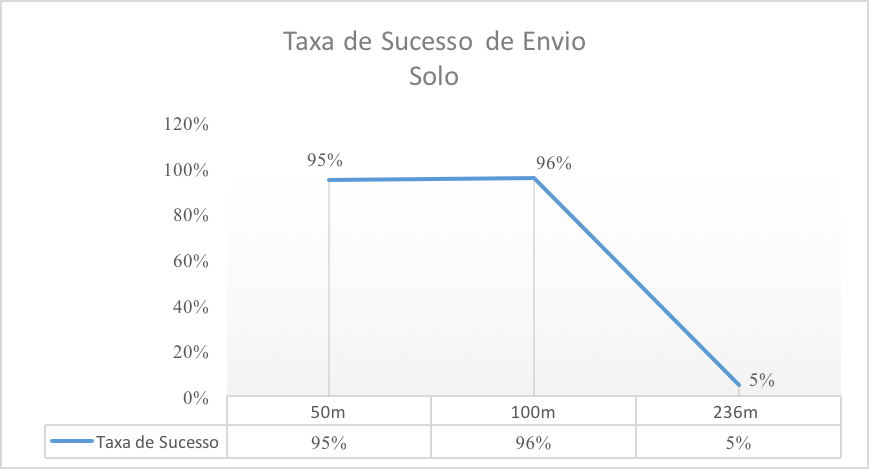
\includegraphics[width=0.7\textwidth]{sucessRateChao.png}
\caption{Gráfico da taxa de sucesso de envio \emph{versus} distância entre os dois nós da rede XBee.} 
\label{fig:SuccessChao}
\end{figure} 

\begin{figure} 
\center
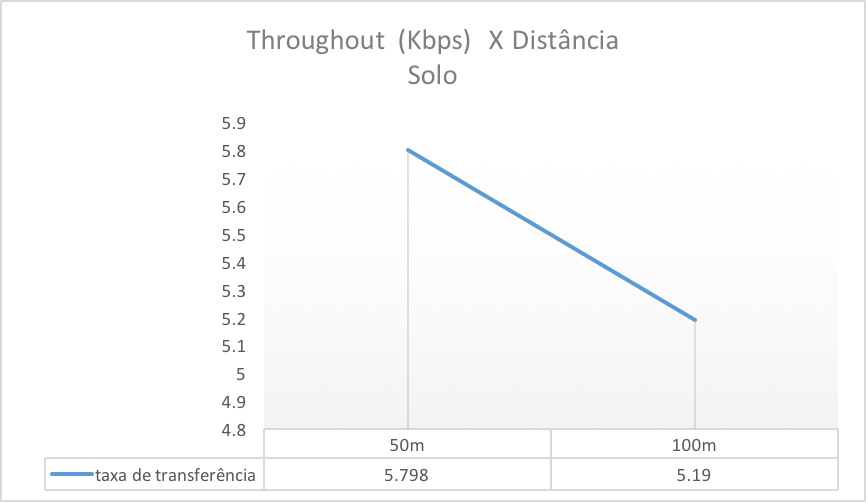
\includegraphics[width=0.7\textwidth]{throughputResultChao.png}
\caption{Gráfico da taxa de transmissão de envio \emph{versus} distância entre os dois nós da rede XBee.} 
\label{fig:ThroughputChao}
\end{figure}
 
\section{Teste em Ar a Distância Fixa}

Os resultados obtidos nos testes realizados em ar foram consistentes com as especificações do módulo XBee. Foram realizados testes de força de sinal e taxa de transmissão com afastamentos entre os nós de 50 até 700 metros e altitude fixada em 80 metros, sendo de 50 a 400 metros com aumentos de 50 metros e de 400 a 700 metros com aumentos de 100 metros.

Para todos os testes realizados, todos os quarenta pacotes enviados, por teste, foram transmitidos com sucesso entre o nó remetente e o nó destinatário, resultando em um taxa de sucesso de envio de cem por cento em toda essa faixa de distância, que vai de 50 até 700 metros de afastamento entre os nós.

Apesar da excelente taxa de sucesso, a potência do sinal transmitido entre os nós teve um comportamento inesperado. Em um cenário de afastamento entre os nós, o valor de RSSI (em português, indicador de potência de sinal recebido) deveria decaí proporcionalmente ao afastamento os nós, resultando em um \emph{link} de conexão mais fraco entre os nós. No entanto, nos resultados do experimento esse indicador varia com a distância de afastamento de forma irregular. Esse comportamento pode ser verificado na figura \ref{fig:RangeChao}, onde é possível observar que o valor apresentado decai até os 350 metros de afastamento, onde tem uma repentina subida, decai mais um pouco até os 400 metros e começa a aumentar novamente. 

Quanto a taxa de transmissão, nos testes realizados em ar, os módulos XBee se comportaram de forma altamente inesperada, variando a taxa de transmissão de dados bruscamente, inicialmente, por razão indefinida. A Figura \ref{fig:ThroughputAr} apresenta os resultados obtidos, onde pode-se observar que a taxa de transmissão tem um aumento repentino a partir dos 350 metros de afastamento entre os nós e permanece aumentando com o afastamento, chegando a atingir um \emph{throughput} de aproximadamente 30 kbps.

Apesar do comportamento inesperado, os testes em ar foram condicentes com as especificações do módulo. Já a respeito do comportamento inesperado, testes preliminares apontaram que fatores como o tamanho do pacote a ser enviado, bem como \emph{baudrate}, possuem grande efeito tanto na taxa de sucesso da comunicação quanto na taxa de transmissão desses pacotes, o que leva a acreditar que a taxa de transmissão de 200 kbps apresentada no manual do módulo XBee poderá vir a ser alcançada mudando alguns parâmetros de configuração do módulo e características do pacote a ser enviado.\\

Os resultados obtidos nesse trabalho foram importantes para direcionar os testes futuros a serem realizados dentro do projeto SpaceVANT e produzir um protocolo de testes mais formalizado levando em consideração os parâmetros que afetam a qualidade da conexão na rede XBee.   

\begin{figure} 
\center
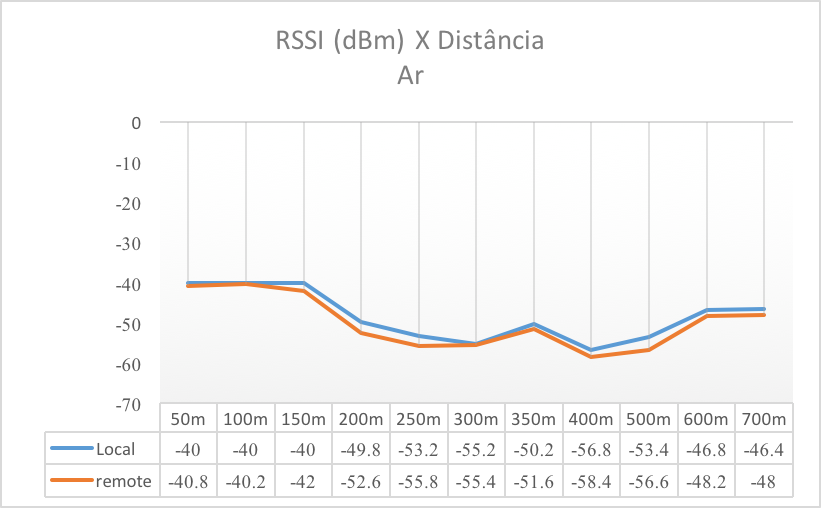
\includegraphics[width=0.7\textwidth]{rangeResultAr.png}
\caption{Gráfico do RSSI local e remoto \emph{versus} distância entre os dois nós da rede XBee.} 
\label{fig:RangeChao}
\end{figure}

\begin{figure} 
\center
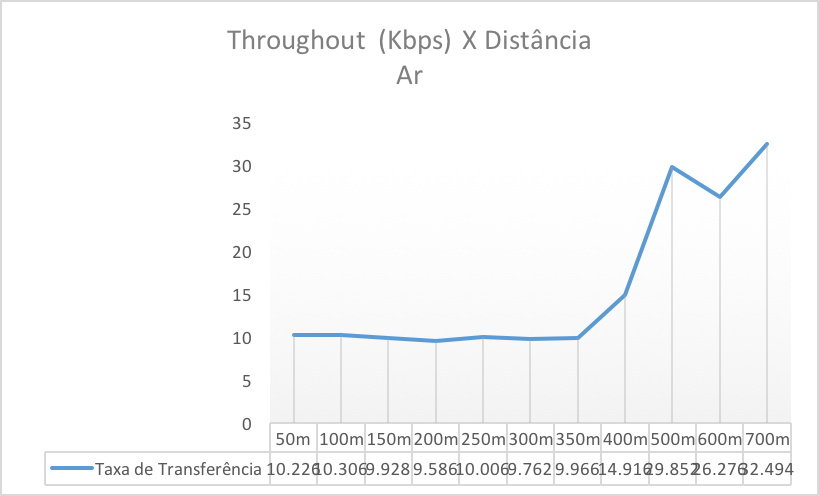
\includegraphics[width=0.7\textwidth]{throughputResultAr.png}
\caption{Gráfico da taxa de transmissão de envio \emph{versus} distância entre os dois nós da rede XBee.} 
\label{fig:ThroughputAr}
\end{figure}










